\section{Simulation Results}
\label{sec:simulations}

\noindent\textit{Working-draft data status:}
GP-MP uses the white-noise-trained networks in
Figs.~\ref{fig:cstmp-denoising}--\ref{fig:cstmp-snr}
and Table~\ref{tab:activity-evidence}; GP-MP-EP in Fig.~\ref{fig:cstmp-snr}
uses the same networks. The GP-MP results in
Figs.~\ref{fig:cstmp-pilots}--\ref{fig:cstmp-cross} use earlier checkpoints
with different training perturbations and await replacement.

\subsection{Simulation Settings}
\label{sec:simulation-settings}

\subsubsection{Channel Dataset and System Parameters}
Table~\ref{tab:simulation-parameters} summarizes the default settings.
Devices are uniformly distributed over the beam footprint, with delays,
Doppler shifts, and array responses determined by the geometry.
Large-scale effects are compensated. We use the NTN-TDL-D profile
\cite{shen2025}, with a delay spread drawn uniformly from $[30,50]$~ns,
a line-of-sight gain of fixed amplitude and uniform phase, and proper
complex Gaussian diffuse gains. Path parameters remain fixed per block.
The training and validation sets contain $50{,}000$ and $5{,}000$ clean
$16\times16\times16$ channels, respectively, drawn from disjoint sets
of scenes. Each scene provides four channel samples before multiplication
by $\alpha_k$.

For $Q\leq KN$, the pilots are constructed from distinct DFT rows
$r_q\in\{0,\ldots,KN-1\}$, with a column permutation
$\{c_{kn}\}_{k,n}$ of the same set and independent phases
$\phi_{kn}\sim\mathcal U[0,2\pi)$:

\begin{equation}
 [\mathbf p_{qk}]_n=\sqrt{\frac{E_p}{N}}
 e^{-\mathrm j2\pi r_qc_{kn}/(KN)}e^{\mathrm j\phi_{kn}},
 \label{eq:pilot}
\end{equation}
with $\sum_{n=0}^{N-1}|[\mathbf p_{qk}]_n|^2=E_p$.

Independent Bernoulli activity variables with nominal probability $p$ are
conditioned on at least one active device. The receiver prior uses the
resulting marginal activity probability $\rho=p/[1-(1-p)^K]$.
The received SNR is the ratio of the average noiseless signal power per
complex observation to the noise variance. The signal power is averaged
over the $QMN$ entries of $\mathbf A\mathbf X$ in each scene, and
$\sigma^2$ is chosen to achieve the specified SNR.

\begin{table}[!t]
\caption{Simulation Parameters}
\label{tab:simulation-parameters}
\centering
\small
\begin{tabular}{@{}ll@{}}
\toprule
Parameter & Value \\
\midrule
Carrier frequency $f_c$ & $2$~GHz \\
Satellite altitude & $600$~km \\
Beam radius & $128$~km \\
Minimum elevation angle & $30^\circ$ \\
UPA dimensions $M_y\times M_z$ & $4\times4$ \\
Array element spacing $d_y,d_z$ & $\lambda/2$ \\
Number of chirp subcarriers $N$ & $16$ \\
Subcarrier spacing $\Delta f$ & $30$~kHz \\
Chirp parameters $(c_1,c_2)$ & $(7/32,1/320)$ \\
CPP length $N_{\rm CPP}$ & $336$ \\
Differential-delay range & $[0,699]~\mu$s \\
Doppler-shift range & $[-41,41]$~kHz \\
Power delay profile & NTN-TDL-D \\
Delay spread & $[30,50]$~ns \\
Rician factor & $11.707$~dB \\
Default $(K,Q,p)$ & $(40,16,0.1)$ \\
\bottomrule
\end{tabular}
\end{table}

\subsubsection{Network Architectures and Training}
\label{sec:network-settings}
\label{sec:training-settings}
The denoiser uses the RefineNet \cite{lin2017} variant in
\cite[Appendix~A]{song2019}, with $2M$ real and imaginary input maps over
$N\times N$ DAFT coordinates.
Each stage contains two residual blocks, each with two
$3\times3$ convolutions, conditional instance normalization, and
exponential linear unit (ELU) activations.
The stage outputs are combined by four refinement blocks that restore
the spatial resolution, with $3\times3$ convolutions at the network
input and output. Table~\ref{tab:network-architectures} lists the channel
widths and spatial resolutions of both networks.

\begin{table}[!t]
\caption{Network Architectures}
\label{tab:network-architectures}
\centering
\small
\setlength{\tabcolsep}{3pt}
\begin{tabular}{@{}lcc@{}}
\toprule
Layer or stage & Channels & Map size \\
\midrule
\multicolumn{3}{@{}l}{\textit{Channel denoiser}} \\
Input convolution & $128$ & $N\times N$ \\
Residual stage 1 & $128$ & $N\times N$ \\
Residual stage 2 & $256$ & $N/2\times N/2$ \\
Residual stage 3 (dilation 2) & $256$ & $N/2\times N/2$ \\
Residual stage 4 (dilation 4) & $256$ & $N/2\times N/2$ \\
Refinement blocks 1--2 & $256,256$ & $N/2\times N/2$ \\
Refinement block 3 & $128$ & $N/2\times N/2$ \\
Refinement block 4 & $128$ & $N\times N$ \\
Output convolution & $2M$ & $N\times N$ \\
\midrule
\multicolumn{3}{@{}l}{\textit{Activity classifier}} \\
Convolutional stage 1 & $64$ & $N\times N$ \\
Convolutional stage 2 & $128$ & $N/2\times N/2$ \\
Convolutional stage 3 & $128$ & $N/4\times N/4$ \\
Fully connected layers & $128,1$ & --- \\
\bottomrule
\end{tabular}
\end{table}

Noise conditioning uses an embedding of $\log(v)/5$, formed by two
$64$-unit fully connected layers with sigmoid-weighted linear unit
(SiLU) activations and linearly projected to the normalization layers.
The denoiser also adopts the preconditioning in \cite[Sec.~5]{karras2022}:

\begin{equation}
 \begin{aligned}
 \mathbf f_\theta(\mathbf u,v)
 &=c_{\rm skip}(v)\mathbf u+c_{\rm out}(v)
   \mathbf g_\theta(c_{\rm in}(v)\mathbf u,v),\\
 c_{\rm in}(v)&=(\sigma_{\rm d}^2+v/2)^{-1/2},\\
 c_{\rm skip}(v)&=\frac{\sigma_{\rm d}^2}{\sigma_{\rm d}^2+v/2},\\
 c_{\rm out}(v)&=\left(\frac{\sigma_{\rm d}^2 v/2}
 {\sigma_{\rm d}^2+v/2}\right)^{1/2}.
 \end{aligned}
 \label{eq:mean-preconditioning}
\end{equation}

Here $\sigma_{\rm d}^2=1/2$ is the nominal variance per real coordinate after
normalization, and $\mathbf g_\theta$ is the RefineNet described above.

The classifier estimates the log likelihood ratio from $4M$ real and
imaginary maps of $\mathbf R$ and $\mathbf F_\theta(\mathbf R,v)$,
scaled by $\sqrt{2/(1+v)}$, together with five scalars:
$\log(v)/5$, logarithmic transforms of input/output/residual energies
normalized by $Dv$, and a sign-preserving logarithmic transform of the
real inner product normalized by $Dv$.
Its three convolutional stages each contain two $3\times3$ convolutions
with SiLU activations and padding $1$. Downsampling uses stride $2$ in
the first convolution of stages~2--3; the remaining convolutions use
stride $1$.
Noise conditioning is provided by a $64$-unit fully connected SiLU
embedding of $\log(v)/5$, whose linear projections are added to the
stage outputs. The flattened features and five scalars are combined by
the fully connected layers in Table~\ref{tab:network-architectures},
with SiLU between them, to produce one logit per device.

Training minimizes \eqref{eq:first-loss} with the preconditioning in
\eqref{eq:mean-preconditioning}, using $v$ sampled uniformly on a
logarithmic scale over $[10^{-3},10^2]$.
The denoiser is optimized using Adam for $200$ epochs with batch size
$64$, initial learning rate $10^{-4}$, and exponential moving average
decay $0.999$. Model selection uses the lowest validation loss under
fixed noise realizations. The STMP reference uses the same clean
channels and number of epochs.

With the denoiser fixed, the classifier is trained from random
initialization by minimizing \eqref{eq:classifier-loss} for $100$ epochs,
with batch size $32$ and initial learning rate $3\times10^{-4}$.
The classifier is also selected by validation loss.
Classifier training and receiver evaluation use white Gaussian noise
with covariance $v\I$.

\subsubsection{Compared Receivers}
\label{sec:compared-receivers}
We evaluate GP-MP and five baselines. All use known phases except
for GP-MP-EP:
\begin{itemize}[leftmargin=*,topsep=2pt,itemsep=2pt,parsep=0pt]
\item \textbf{GP-MP:} The proposed receiver; EP denotes estimated phases.
\item \textbf{STMP:} We adapt STMP \cite{cai2026} to the multi-frame
AFDM model, retaining its white-noise-trained first- and second-order
score networks for conditional mean and variance estimation. We replace
its Gaussian-message-based activity-probability update with a learned
density-ratio estimator trained using the corresponding first-order network.
\begin{samepage}
\item \textbf{Simultaneous orthogonal matching pursuit (SOMP):}
\cite{TroppGilbertStrauss2006SOMP}
This greedy method sequentially selects
dictionary atoms shared by the receive antennas and estimates their
coefficients by least squares. We use an integer delay--Doppler dictionary
and select up to $64$ atoms.
\par
\end{samepage}
\item \textbf{GAMP-SBL:} This method uses generalized approximate message
passing in sparse Bayesian learning \cite{ZhangFanHaoQuan2023GAMPSBL}.
Our implementation uses the integer delay--Doppler dictionary,
shares row precisions across receive antennas, and allows up to
$1{,}000$ iterations.
\item \textbf{GNN-ASPL:} This method alternates AMP-based channel estimation
with adaptive sparsity pattern learning using a graph neural network
\cite{ding2026}. It uses the same integer delay--Doppler dictionary and
a $10$-layer network.
\item \textbf{Off-grid SBL:} In addition to the channel coefficients,
this method estimates continuous delay and Doppler offsets through a
first-order linear approximation of the dictionary
\cite{WeiEtAl2022OffgridSBL}. We allow up to $120$ iterations.
For the SNR comparison, the $7$, $13$, and $25$ Doppler grid points
are paired with $12$, $24$, and $48$ retained candidates per device
and $48$, $96$, and $192$ offset candidates per iteration, respectively;
all three configurations use $112$ delay grid points.
\end{itemize}

\begin{table}[!t]
\caption{Activity Detection Performance and Iteration-Limit Rates}
\label{tab:activity-evidence}
\centering
\small
\setlength{\tabcolsep}{2pt}
\begin{tabular}{@{}rcccccccc@{}}
\toprule
& \multicolumn{4}{c}{STMP}
& \multicolumn{4}{c}{GP-MP} \\
\cmidrule(lr){2-5}\cmidrule(l){6-9}
& \multicolumn{2}{c}{Gaussian} & \multicolumn{2}{c}{Density ratio}
& \multicolumn{2}{c}{Gaussian} & \multicolumn{2}{c}{Density ratio} \\
\cmidrule(lr){2-3}\cmidrule(lr){4-5}\cmidrule(lr){6-7}\cmidrule(l){8-9}
\shortstack{SNR\\(dB)} & \shortstack{AER\\(\%)} & \shortstack{Limit\\(\%)}
& \shortstack{AER\\(\%)} & \shortstack{Limit\\(\%)}
& \shortstack{AER\\(\%)} & \shortstack{Limit\\(\%)}
& \shortstack{AER\\(\%)} & \shortstack{Limit\\(\%)} \\
\midrule
$-4$ & $9.225$ & $2$ & $0.525$ & $0$ & $44.575$ & $63$ & $0.200$ & $0$ \\
$-2$ & $7.875$ & $3$ & $0.225$ & $0$ & $43.475$ & $55$ & $0.125$ & $0$ \\
$0$ & $6.375$ & $2$ & $0.100$ & $0$ & $40.975$ & $46$ & $0.075$ & $0$ \\
$2$ & $5.550$ & $1$ & $0.050$ & $0$ & $36.750$ & $31$ & $0.025$ & $0$ \\
$4$ & $4.800$ & $1$ & $0.025$ & $0$ & $32.050$ & $19$ & $0.025$ & $0$ \\
$6$ & $4.225$ & $0$ & $0.025$ & $0$ & $27.425$ & $11$ & $0.025$ & $0$ \\
\bottomrule
\end{tabular}
\end{table}

\subsubsection{Evaluation Settings and Metrics}
\label{sec:receiver-settings}
\label{sec:stopping-criteria}
Phase estimation in GP-MP-EP covers $d\in[0,N)$ and
$|\nu|\leq\nu_{\max}$, where $\nu_{\max}$ is the channel model's Doppler
bound. Pilot correlations over $128$ phase bins identify three coarse
candidates. The Doppler values corresponding to each candidate phase
within this bound form the initial search set, from which the best
$12$ are refined by at most $25$ L-BFGS-B iterations per candidate
within a differentiable interval of the waveform. Coordinate refinement
starts from zero powers and uses two sweeps in descending order of
initial pilot-correlation scores, with the current parameters retained
among the candidates.

All receivers estimate the noise variance from the observations.
STMP and GP-MP use activity threshold $0.5$ and default damping factors
of $0.2$ and $0.4$, respectively.
Their iterations are bounded by $I_{\min}=60$ and $I_{\max}=600$,
with relative-change tolerance $5\times10^{-4}$.
After $I_{\min}$ iterations, convergence is assessed from the stability
of channel and activity estimates and the consistency of variance
updates. Runs that reach $I_{\max}$ return the last iterate.
\ifdefined\FullManuscript
The complete stopping checks and tolerances are given in
Appendix~\ref{app:implementation-settings}.
\fi

GP-MP uses $L_z=1$ and $\delta_{\rm FD}=10^{-2}$ in
\eqref{eq:derivative-trace}, with the random sign vectors reused across
iterations. The common variance has a lower bound $\tau_{\min}=10^{-4}$.

Receiver comparisons use paired scenes, with the same scenes reused
across conditions. Each SNR point uses $1{,}000$ scenes, whereas each
point in the pilot-frame, device-count, activity-probability, and
cross-profile figures uses $500$ scenes.
The activity-update comparison in Table~\ref{tab:activity-evidence}
uses $100$ paired scenes per SNR.
\ifdefined\FullManuscript
Appendix~\ref{app:evaluation-protocol} gives the evaluation protocol.
\fi

For scene indices $e\in\mathcal T$ at a given condition, the
normalized mean-squared error (NMSE) is the sum of squared Frobenius
errors between $\widehat{\mathbf X}_{ek}$ and $\mathbf X_{ek}$, divided
by the sum of squared Frobenius norms of $\mathbf X_{ek}$.
Both sums cover all scenes in $\mathcal T$ and all $K$ devices, including
inactive devices; the ratio is reported in decibels.
For direct channel denoising, $\mathbf X$ is replaced by
$\mathbf H$ and the sums run over individual channel samples.
The activity error rate (AER) is the total number of missed detections
and false alarms divided by the $K|\mathcal T|$ device decisions.

\begin{figure}[!t]
\centering
\makebox[\columnwidth][c]{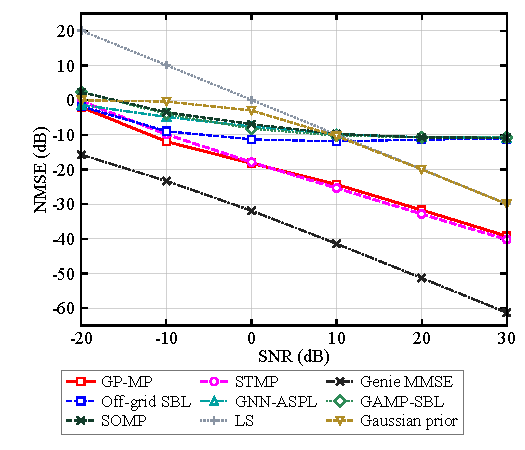
\includegraphics[width=88.9mm]{channel_denoising.pdf}}
\caption{Channel denoising under AWGN with known variance.}
\label{fig:cstmp-denoising}
\end{figure}

\begin{figure}[!t]
\centering
\makebox[\columnwidth][c]{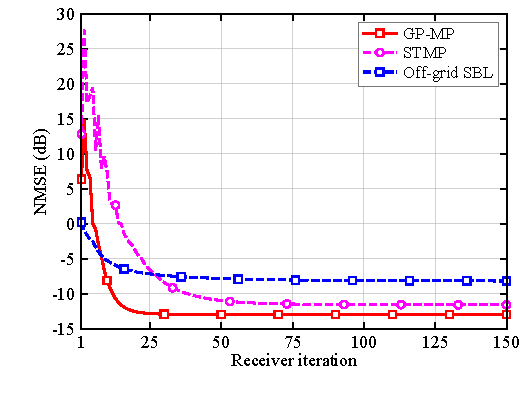
\includegraphics[width=88.9mm]{convergence.pdf}}
\caption{NMSE versus iteration over $30$ paired scenes at
$0$~dB, with $K=40$, $Q=16$, and $p=0.1$.}
\label{fig:cstmp-convergence}
\end{figure}

\begin{figure}[!t]
\centering
\makebox[\columnwidth][c]{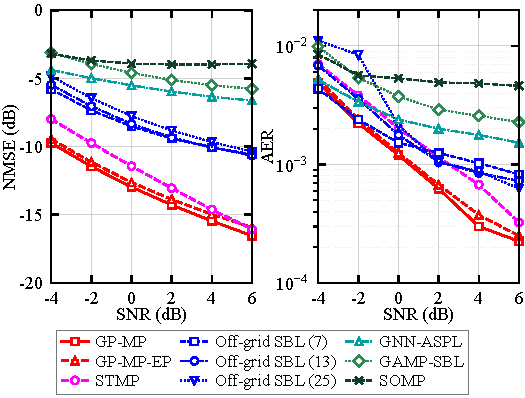
\includegraphics[width=88.9mm]{snr_comparison.pdf}}
\caption{Channel NMSE and AER versus SNR with $K=40$, $Q=16$, and
$p=0.1$, using $1{,}000$ paired scenes per point. Numbers in the
Off-grid SBL labels indicate the Doppler grid points.}
\label{fig:cstmp-snr}
\end{figure}

\begin{figure}[!t]
\centering
\makebox[\columnwidth][c]{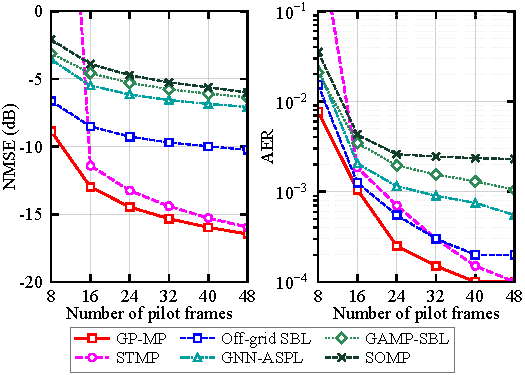
\includegraphics[width=88.9mm]{pilot_frames.pdf}}
\caption{Channel NMSE and AER versus the number of pilot frames at
$0$~dB, with $K=40$ and $p=0.1$.}
\label{fig:cstmp-pilots}
\end{figure}

\begin{figure}[!t]
\centering
\makebox[\columnwidth][c]{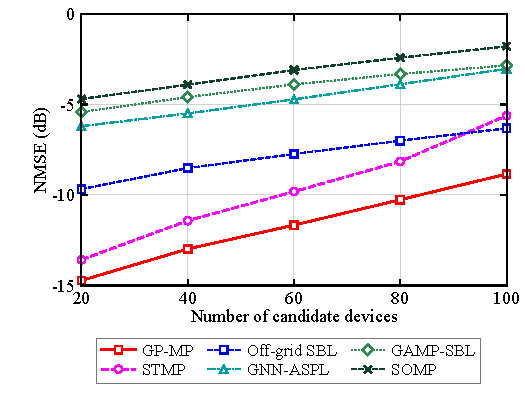
\includegraphics[width=88.9mm]{user_count.pdf}}
\caption{Channel NMSE versus the number of candidate devices
at $0$~dB, with $Q=16$ and $p=0.1$.}
\label{fig:cstmp-users}
\end{figure}

\begin{figure}[!t]
\centering
\makebox[\columnwidth][c]{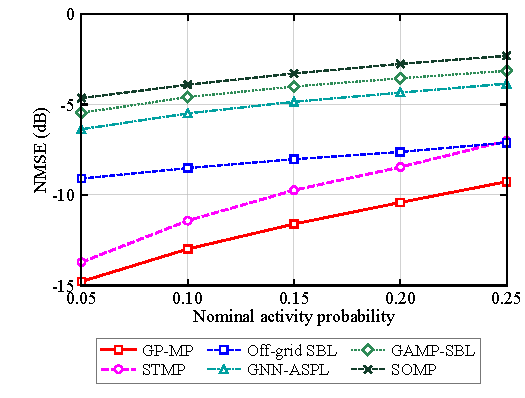
\includegraphics[width=88.9mm]{activity_probability.pdf}}
\caption{Channel NMSE versus nominal activity probability at
$0$~dB, with $K=40$ and $Q=16$.}
\label{fig:cstmp-activity}
\end{figure}

\begin{figure*}[!t]
\centering
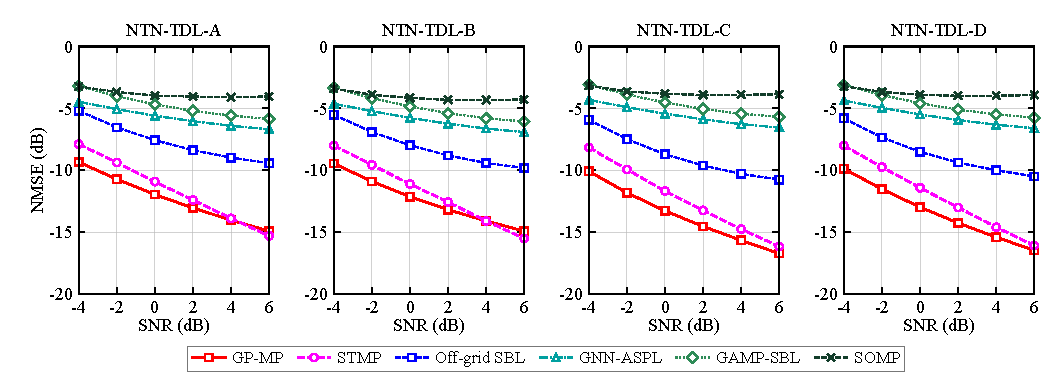
\includegraphics[width=177.8mm]{cross_channel.pdf}
\caption{Channel NMSE for NTN-TDL profiles A, B, C, and D (from left
to right). Each point uses $500$ paired physical scenes, $K=40$,
$Q=16$, and $p=0.1$. The learned receivers are trained
on profile D and evaluated without retraining.}
\label{fig:cstmp-cross}
\end{figure*}

\subsection{Channel Denoising Performance}
\label{sec:denoising-performance}
Following \cite[Sec.~VI-B]{cai2026}, we first assess channel denoising
under AWGN using $\mathbf R=\mathbf H+\mathbf W$, with
$\vect(\mathbf W)\sim\CN(\mathbf0,v\I)$, known $v$, and nominal SNR
$-10\log_{10}v$. At each of six SNRs from $-20$ to $30$~dB, both
neural estimators use the same $2{,}000$ samples from $500$ scenes and
the same white-noise realizations. The following reference methods are included:
\begin{itemize}[leftmargin=*,topsep=2pt,itemsep=2pt,parsep=0pt]
\item \textbf{Least squares (LS):} The estimate is the noisy observation
$\mathbf R$.
\item \textbf{Gaussian-prior estimate:} The estimate is
$\widehat P_H\mathbf R/(\widehat P_H+v)$, where $\widehat P_H$ is the
training-channel power defined in Section~\ref{sec:schedule}.
\item \textbf{Genie-aided conditional MMSE:} We compute the analytic
conditional MSE of the remaining Gaussian gains given the true path
geometry, powers, and line-of-sight gain.
\end{itemize}
The four sparse-recovery methods in Section~\ref{sec:compared-receivers}
are also evaluated using an identity observation operator and known AWGN
variance. They retain their receiver settings and GNN weights;
GAMP-SBL retains its internal noise-variance update.

In Fig.~\ref{fig:cstmp-denoising}, both learned denoisers outperform LS
and the Gaussian-prior estimate across the evaluated range.
Their NMSE continues to decrease with SNR, whereas the four sparse-recovery
methods approach error floors, leaving a wider gap at moderate and high SNR.
The GP-MP denoiser has lower NMSE at low SNR,
whereas the STMP denoiser is more accurate at high SNR.
Both learned denoisers have higher NMSE than the genie-aided reference,
which uses true path information.

\subsection{Effect of Density Ratio Estimation}
\label{sec:activity-evidence}
The effect of density ratio estimation is evaluated by comparing the
learned activity update with the Gaussian approximation, for which

\begin{align}
 \ell_k^{\rm G}&=\frac{\norm{\mathbf R_k}_F^2}{v}
 -\frac{\norm{\mathbf R_k-\mathbf E_k}_F^2}{\tau_k^{\rm ext}+v}
 \notag\\
 &\quad-D\log\left(1+\frac{\tau_k^{\rm ext}}{v}\right),
 \label{eq:gaussian-evidence}\\
 p_k&=\sigmoid(\logit\rho+\ell_k^{\rm G}).
 \label{eq:gaussian-activity}
\end{align}

Each receiver, STMP and GP-MP, is evaluated with both activity updates
under otherwise identical settings. The two GP-MP variants share the
white-noise-trained denoiser, with the matched classifier used for
density ratio estimation. Table~\ref{tab:activity-evidence} reports AER
over all runs and the percentage reaching the $600$-iteration limit
(Limit).

For both receivers, the learned density ratio gives lower AER at every
evaluated SNR, with no runs reaching the iteration limit. With the
Gaussian approximation, STMP has lower AER than GP-MP throughout the
evaluated range and reaches the iteration limit less frequently. The
comparison therefore supports the use of learned density ratios in
both receivers, with a larger improvement for GP-MP.

\subsection{JADCE Performance}
\label{sec:jadce-performance}
Unless stated otherwise, the receivers use the defaults in
Table~\ref{tab:simulation-parameters} and the evaluation settings in
Section~\ref{sec:receiver-settings}.

Figure~\ref{fig:cstmp-convergence} compares the NMSE trajectories of
GP-MP, STMP, and Off-grid SBL over $30$ paired scenes, with early
stopping disabled. GP-MP approaches a lower NMSE in fewer iterations
than STMP, while Off-grid SBL levels off at a higher NMSE.

Figure~\ref{fig:cstmp-snr} compares channel NMSE and AER over
$-4$ to $6$~dB. GP-MP achieves the lowest NMSE throughout this range.
Its advantage over STMP is more pronounced at low SNR and narrows as
SNR increases. At $0$~dB, GP-MP achieves an NMSE approximately
$1.5$~dB lower than STMP. Off-grid SBL has the lowest NMSE among the four
sparse-recovery baselines. The NMSE of these baselines decreases more
slowly with SNR than that of the learned receivers, so the gap between
the two groups grows.

The AER also generally decreases with SNR. GP-MP has lower AER than
STMP throughout the range and outperforms the four sparse-recovery
baselines at moderate and high SNR.

With estimated phases, GP-MP-EP incurs an NMSE increase of
$0.28$--$0.60$~dB relative to GP-MP over the evaluated SNR range,
while its AER remains close to the known-phase reference.

Figure~\ref{fig:cstmp-pilots} shows the effect of the number of pilot frames.
Additional frames provide further observations of the same effective
channels at fixed per-frame energy, and generally improve both channel
estimation and activity detection. Among the evaluated frame counts,
GP-MP first reaches $-14$~dB NMSE at $Q=24$, whereas STMP requires
$Q=32$. This corresponds to $25\%$ fewer pilot frames for the same
NMSE target.

Figure~\ref{fig:cstmp-users} compares the channel NMSE for $K=20$--$100$.
At fixed activity probability and pilot-frame count, increasing $K$
enlarges the set of candidate channels and raises the expected number
of active devices. All methods exhibit higher NMSE as this load increases.
GP-MP maintains the lowest NMSE, and its advantage over STMP grows
with the number of candidate devices.

Figure~\ref{fig:cstmp-activity} examines the effect of increasing the
nominal activity probability from $0.05$ to $0.25$ with a fixed candidate
set. With fixed pilot and antenna resources, more active channels must
be recovered, and all methods exhibit higher NMSE. GP-MP retains
the lowest NMSE, and its advantage over STMP increases with activity
probability.

\subsection{Comparison Across Channel Profiles}
Performance beyond the training distribution is evaluated on NTN-TDL
profiles A, B, and C using the networks trained on profile D without
retraining. These evaluations vary the power delay profiles and fading
distributions while retaining the geometry, pilots, and receiver
settings, with $500$ paired scenes per condition.

Figure~\ref{fig:cstmp-cross} shows that GP-MP achieves lower NMSE than
the four sparse-recovery baselines on every evaluated profile.
This result indicates that the learned effective-channel prior remains
useful beyond the training profile. The difference relative to STMP
is smaller and varies with the profile and SNR.
